% Section content template for individual Educative lessons
% This file contains the actual content for a specific section
% Generated from Educative API section content

% Section: Design of a CDN
% Section ID: 5883973992972288
% Section Slug: design-of-a-cdn
% Generated: 2025-12-07T17:13:19.718668

\subsection{CDN design}\label{d11H4s3yYA4u1yAulvVrq}
\\
We'll explain our CDN design in two phases. In the first phase, we'll cover the components that comprise a CDN. By the end of this phase, we'll understand why we need a specific component. In the second phase, we'll explore the workflow by explaining how each component interacts with others to develop a fully functional CDN. Let 's dive in.

\subsubsection{CDN components}\label{zifrggvnSXnm4aYOWEA_T}
\\
The following components comprise a CDN:

\begin{itemize}
\item
\protect\phantomsection\label{6zTS9TpzgelKH-7kHE8Yr}
\textbf{Clients}: End users use various clients, like browsers, smartphones, and other devices, to request content from the CDN.
\item
\protect\phantomsection\label{2k4ua4qWy8FbOcYKsvydG}
\textbf{Routing system}: The routing system directs clients to the nearest CDN facility. To do that effectively, this component receives input from various systems to understand where content is placed, how many requests are made for particular content, the load a particular set of servers is handling, and the URI (Uniform Resource Identifier) namespace of various contents. In the next lesson, we'll discuss different routing mechanisms to forward users to the nearest CDN facility.
\item
\protect\phantomsection\label{JEdlxtwBDNqrakP0wK7Xp}
\textbf{Scrubber servers}: Scrubber servers are used to separate the good traffic from malicious traffic and protect against well-known attacks, like DDoS. Scrubber servers are generally used only when an attack is detected. In that case, the traffic is scrubbed or cleaned and then routed to the target destination.
\item
\protect\phantomsection\label{Sk3uyUCcv-6oatRzp2EPl}
\textbf{Proxy servers}: The proxy or edge proxy servers serve the content from RAM to the users. Proxy servers store hot data in RAM, though they can store cold data in SSD or hard drive as well. These servers also provide accounting information and receive content from the distribution system.
\item
\protect\phantomsection\label{X8hHnJQMUYc2FmwqRxOim}
\textbf{Distribution system}: The distribution system is responsible for distributing content to all the edge proxy servers to different CDN facilities. This system uses the Internet and intelligent broadcast-like approaches to distribute content across the active edge proxy servers.
\item
\protect\phantomsection\label{f-fobCj0CB6uVvUAyR0FW}
\textbf{Origin servers}: The CDN infrastructure facilitates users with data received from the origin servers. The origin servers serve any unavailable data at the CDN to clients. Origin servers will use appropriate stores to keep content and other mapping metadata. Though, we won't discuss the internal architecture of origin infrastructure here.
\item
\protect\phantomsection\label{V6ZIUMOBwe4q2N-lV1cCw}
\textbf{Management system}: The management systems are important in CDNs from a business and managerial aspect where resource usage and statistics are constantly observed. This component measures important metrics, like latency, downtime, packet loss, server load, and so on. For third-party CDNs, accounting information can also be used for billing purposes.
\end{itemize}

\begin{figure}[htbp]
 \centering
 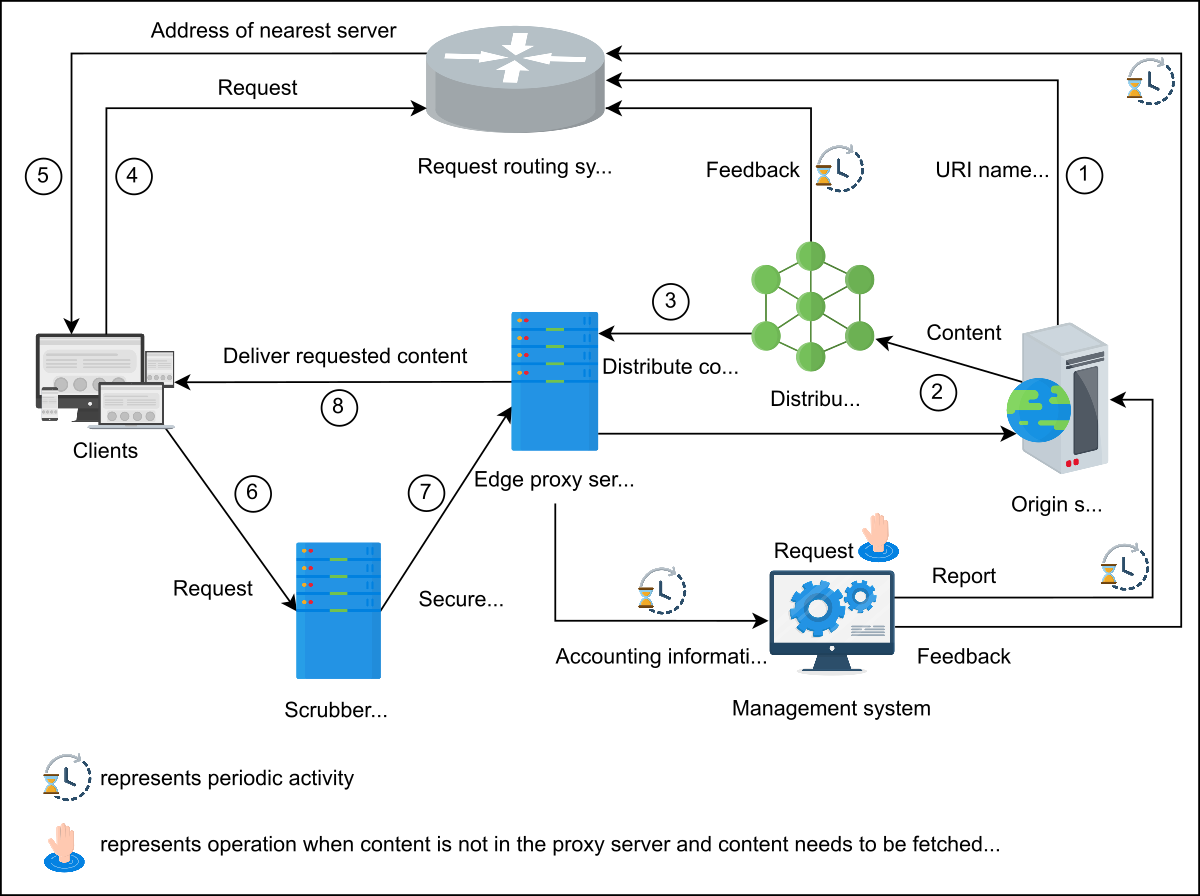
\includegraphics[width=0.5\textwidth]{Images/chapter_11/section_5883973992972288/5105434411401216.png}
 \caption{CDN components}
\end{figure}

\subsubsection{Workflow}\label{81fJJznjuyomO2paSwX2s}
\\
The workflow for the abstract design is given below:

\begin{enumerate}
\item
\protect\phantomsection\label{ZG8Ypcc_mJ0-JrGI8ujMi}
The origin servers provide the URI namespace delegation(URI namespace delegation is the process of assigning control of different parts of a URI namespace (such as domain name) to a particular organization.) of all objects cached in the CDN to the request routing system.
\item
\protect\phantomsection\label{C9hfZoq2EtGg2rQbyVl3x}
The origin server publishes the content to the distribution system responsible for data distribution across the active edge proxy servers.
\item
\protect\phantomsection\label{rkGCUme0uQ3tfujUBevjZ}
The distribution system distributes the content among the proxy servers and provides feedback to the request routing system. This feedback is helpful in optimizing the selection of the nearest proxy server for a requesting client. This feedback contains information about which content is cached on which proxy server to route traffic to relevant proxy servers.
\item
\protect\phantomsection\label{vTtMTr-iLTrDWLNPILMJc}
The client requests the routing system for a suitable proxy server from the request routing system.
\item
\protect\phantomsection\label{zCeUNLByyNc1miFKXQFi0}
The request routing system returns the IP address of an appropriate proxy server.
\item
\protect\phantomsection\label{joKGNLqeTnPUn3-zoH7Op}
The client request routes through the scrubber servers for security reasons.
\item
\protect\phantomsection\label{3mymZgaQe6EMTzoso7icD}
The scrubber server forwards good traffic to the edge proxy server.
\item
\protect\phantomsection\label{qWCQ44UeMxI2OeWrkkEVo}
The edge proxy server serves the client request and periodically forwards accounting information to the management system. The management system updates the origin servers and sends feedback to the routing system about the statistics and detail of the content. However, the request is routed to the origin servers if the content isn't available in the proxy servers. It 's also possible to have a hierarchy of proxy servers if the content isn't found in the edge proxy servers. For such cases, the request gets forwarded to the parent proxy servers.
\end{enumerate}

\subsection{API Design}\label{O5demcRxasRAWWTBf7GH_}
\\
This section will discuss the API design of the functionalities offered by CDN. This will help us understand how the CDN will receive requests from the clients, receive content from the origin servers, and communicate to other components in the network. Let 's develop APIs for each of the following functionalities:

\begin{itemize}
\item
\protect\phantomsection\label{hKu-u_HIVyFG4OT8Zoqap}
Retrieve content
\item
\protect\phantomsection\label{ZwliNr3Gmgpi4DnYf3HSP}
Deliver content
\item
\protect\phantomsection\label{_g0fhtZWNyvT_flTUNCGJ}
Request content
\item
\protect\phantomsection\label{99nCdS4HQtpIyeO8rf2O3}
Search content
\item
\protect\phantomsection\label{aNKtKnGs64u-qa1CjSaN1}
Update content
\item
\protect\phantomsection\label{hUxqNMuzrlRyZK8UEItwm}
Delete content
\end{itemize}
\\
Content can be anything, like a file, video, audio, or other web object. Here , we'll use the word ``content'' to refer to all of the above. For clarity, we won't discuss the privacy-related parameters---like if the content is public or private, who should be able to access this content, if it should be encrypted, and so on---in the following APIs.

\subsubsection{Retrieve (proxy server to origin server)}\label{O3WDTRjpD3wSc-02ZGViu}
\\
If the proxy servers request content, the \texttt{GET} method retrieves the content through the \texttt{/retrieveContent} API below:

\begin{lstlisting}[language=JavaScript]
retrieveContent(proxyserver_id, content_type, content_version, description)
\end{lstlisting}

Let's see the details of the parameters:

\textbf{Details of Parameters}

\begin{table}[htbp]
\centering
\small
\adjustbox{max width=\textwidth}{
\begin{tabular}{|p{0.198\textwidth}|p{0.752\textwidth}|}
\hline
\textbf{Parameter} & \textbf{Description} \\
\hline
\hline
\texttt{proxyserver\_id} & This is a unique ID of the requesting proxy server. \\
\hline
\texttt{content\_type} & This data structure will contain information about the requested content. Specifically, it will contain the category (audio, video, document, script, and so on), the type of clients it's requested for, and the requested quality (if any). \\
\hline
\texttt{content\_version} & This represents the version number of the content. For the \texttt{/retrieveContent} API, the \texttt{content\_version} will contain the current version of the content residing in the proxy server. The \texttt{content\_version} will be \texttt{NULL} if no previous version is available at the proxy server. \\
\hline
\texttt{description} & This specifies the content detail---for example, the video\textquotesingle s extension, resolution detail, and so on if the \texttt{content\_type} is video. \\
\hline
\end{tabular}
}
\caption{Details of Parameters}
\end{table}

The above API gives a response in a JSON file, which contains the text, content types, links to the images or videos in the content, and so on.

\begin{verbatim}
"Object_links": [ {
"name": "videos" "link": https://app_server.com/api/assets/videos/
}, {
"name": "illustrations" "link": https://app_server.com/api/assets/illustrations/
}, ]
\end{verbatim}

\subsubsection{Deliver (origin server to proxy servers)}\label{b0bLE14dWzRV1h9yPhlEz}
\\
The origin servers use this API to deliver the specified content, the updated version, to the proxy servers through the distribution system. We call this the \texttt{/deliverContent} API:

\begin{lstlisting}[language=JavaScript]
deliverContent(origin_id, server_list, content_type, content_version, description)
\end{lstlisting}

\textbf{Details of Parameters}

\begin{table}[htbp]
\centering
\small
\adjustbox{max width=\textwidth}{
\begin{tabular}{|p{0.202\textwidth}|p{0.748\textwidth}|}
\hline
\textbf{Parameter} & \textbf{Description} \\
\hline
\hline
\texttt{origin\_id} & This recognizes each origin server uniquely. \\
\hline
\texttt{server\_list} & This identifies the list of servers the content will be pushed to by the distribution system. \\
\hline
\texttt{content\_version} & This represents the updated version of the content at the origin server. The proxy server receiving the content will discard the previous version. \\
\hline
\end{tabular}
}
\caption{Details of Parameters}
\end{table}

The rest of the parameters have been explained above already.

\subsubsection{Request (clients to proxy servers)}\label{Y8ZfCc6V7tWyZxpdKvi1G}
\\
The users use this API to request the content from the proxy servers. We call this the \texttt{/requestContent} API:

\begin{lstlisting}[language=JavaScript]
requestContent(user_id, content_type, description)
\end{lstlisting}

\textbf{Details of Parameter}

\begin{table}[htbp]
\centering
\small
\adjustbox{max width=\textwidth}{
\begin{tabular}{|p{0.236\textwidth}|p{0.714\textwidth}|}
\hline
\textbf{Parameter} & \textbf{Description} \\
\hline
\hline
\texttt{user\_id} & This is the unique ID of the user who requested the content. \\
\hline
\end{tabular}
}
\caption{Details of Parameter}
\end{table}

\hfill\break
The specified proxy server returns the particular content to the requested users in response to the above API.

\begin{verbatim}
"Object_links": [
{
	"name": "components"
	"link": https://cdn.app_server.com/api/components/
},
{
	"name": "css"
	"link": https://cdn.app_server.com/api/css/
},
{
	"name": "illustrations"
	"link": https://cdn.app_server.com/api/assets/illustrations/
},
{
	"name": "videos"
	"link": https://cdn.app_server.com/api/assets/videos/
},
{
	"name": "icons"
	"link": https://cdn.app_server.com/api/icons/
},
{
	"name": "fonts"
	"link": https://cdn.app_server.com/api/fonts/
},
]
\end{verbatim}

\subsubsection{Search (proxy server to peer proxy servers)}\label{6HJxs45LVbGqft6o4Hs8M}
\\
Although the content is first searched locally at the proxy server, the proxy servers can also probe requested content in the peer proxy servers in the same PoP(In the context of Content Delivery Networks (CDNs), a Point of Presence (PoP) is a strategically located data center or network access point that serves as a key node for content distribution and delivery. Po Ps are an integral part of a CDN's infrastructure and play a crucial role in optimizing the delivery of web content, including web pages, images, videos, and other digital assets, to end-users.) through the \texttt{/searchContent} API. This could flood the query to all proxy servers in a PoP. Alternatively
, we can use a data store in the PoP to query the content, though proxy servers will need to maintain what content is available on which proxy server.
\\
The \texttt{/searchContent} API is shown below:

\begin{lstlisting}[language=JavaScript]
searchContent(proxyserver_id, content_type, description)
\end{lstlisting}

\subsubsection{Update (proxy server to peer proxy servers)}\label{9Kzdowj3EQVrkoGSDuK_1}
\\
The proxy servers use the \texttt{/updateContent} API to update the specified content in the peer proxy servers in the PoP. It does so when specified isolated scripts run on the CDN to provide image resizing, video resolution conversion, security, and many more services. This type of scripting is known as serverless scripting.
\\
The \texttt{/updateContent} API is shown below:

\begin{lstlisting}[language=JavaScript]
updateContent(proxyserver_id, content_type, description)
\end{lstlisting}

\textbf{Details of Parameter}

\begin{table}[htbp]
\centering
\small
\adjustbox{max width=\textwidth}{
\begin{tabular}{|p{0.236\textwidth}|p{0.714\textwidth}|}
\hline
\textbf{Parameter} & \textbf{Description} \\
\hline
\hline
\texttt{proxyserver\_id} & This recognizes the proxy server uniquely in the PoP to update the content. \\
\hline
\end{tabular}
}
\caption{Details of Parameter}
\end{table}

The rest of the parameters have been explained above already.
\begin{quote}
\textbf{Note}: The Delete API isn't discussed here. In our caching chapter, we discussed different eviction mechanisms in detail. Those mechanisms are also applicable for a CDN content eviction. Nevertheless, situations can arise where the Delete APIs may be required. We'll discuss a few content consistency mechanisms, like how much time content stays in the cache, in the next lesson.
\end{quote}

In the upcoming lessons, we'll dive deep into the characteristics of CDNs.

% End of section content